\documentclass{article}
\usepackage[utf8]{inputenc}
\usepackage[spanish]{babel}
\usepackage{graphicx}
\usepackage{anysize}
\usepackage{fancyhdr} 
\usepackage[export]{adjustbox}
\usepackage{titlesec}
\usepackage{enumitem}
\usepackage{amsmath}
\usepackage{amssymb}
\usepackage{listings}
\usepackage{xcolor}
% \usepackage{hyperref}
% \usepackage{float}
% \usepackage{tabu}

% Izquierda, derecha, arriba, abajo
\marginsize{1.5cm}{2cm}{1.2cm}{1cm} 
\renewcommand{\familydefault}{\sfdefault}
\decimalpoint%

\graphicspath{{assets/}{bdd_prac_05.assets/}}

\setlength{\parindent}{0in}
\titleformat*{\section}{\large\bfseries}

% Para insert código
\definecolor{codegreen}{rgb}{0,0.6,0}
\definecolor{codegray}{rgb}{0.5,0.5,0.5}
\definecolor{codepurple}{rgb}{0.58,0,0.82}
\definecolor{backcolour}{rgb}{1,1,1}

\usepackage{textcomp}
\lstset{upquote=true}
\lstdefinestyle{mystyle}{
    backgroundcolor=\color{backcolour},   
    commentstyle=\color{codegreen},
    keywordstyle=\color{magenta},
    numberstyle=\tiny\color{codegray},
    stringstyle=\color{codepurple},
    basicstyle=\ttfamily\footnotesize,
    breakatwhitespace=false,         
    breaklines=true,                 
    captionpos=b,                    
    keepspaces=true,                 
    % numbers=left,                    
    % numbersep=5pt,                  
    showspaces=false,                
    showstringspaces=false,
    showtabs=false,                  
    tabsize=2
}

\lstset{style=mystyle}

\newcommand{\materia}{BDD}
\newcommand{\clave}{2947}
\newcommand{\profesor}{Ing. Rodriguez Campos \textsc{Jorge Alberto}}
\newcommand{\grupo}{1}
\newcommand{\semestre}{2021-1}

\newcommand{\alumno}{
    Francisco Pablo \textsc{Rodrigo}  \\ 
    Flores Martinez \textsc{Emanuel}   
}

\newcommand{\actividad}{Práctica 05}
\newcommand{\titulo}{Implementación del esquema de fragmentación}

\newcommand{\fechaEntrega}{6 noviembre de 2020}

%%%%%%%%%%%%%%%%%%%% ENCABEZADO %%%%%%%%%%%%%%%%%%%%%%%%%%%%
\pagestyle{fancy}
\fancyhf{}
\renewcommand{\headrulewidth}{0pt}
\fancyhead[R]{% Left header
    \begin{tabular}{l}
        \materia \\ 
        \actividad%
    \end{tabular}
    \,% Space
    \rule[-1.75\baselineskip]{0pt}{0pt}
    % Strut to ensure a 1/4 \baselineskip between image and header rule
    
\includegraphics[height=3\baselineskip,valign=c]{unam}
}
\setlength{\headsep}{0.3in}


\begin{document}
%%%%%%%%%%%%%%%%%%% DATOS PORTADA %%%%%%%%%%%%%%%%%%%%%%%%
\thispagestyle{empty}
\begin{minipage}[t][5cm][t]{0.2\linewidth}
    
\includegraphics[width=2.5cm]{unam.jpg}
    \vspace{10cm}

    
\includegraphics[width=2.5cm]{fiblack}
\end{minipage}
\begin{minipage}[t]{0.7\linewidth}
    \vspace{-2.5cm}
    \LARGE{\textbf{Universidad Nacional Autónoma de México}}\\
    \Large{\textbf{Facultad de Ingeniería}} \\

    \large{\semestre}\\[2cm]

    \large{\textbf{\materia (\clave)}}\\
    \large{\textbf{Gpo: 1}}\\[5mm]
    \large{\textbf{Profesor:} \profesor}\\ [1.5cm]
    \begin{center}
        \LARGE{\textbf{\actividad}}\\
        \LARGE{\textbf{\titulo}}\\
    \end{center}

    \vspace{3.3cm}

    % \large{\textbf{Alumno:} \alumno} \\[1.5cm]
    \large{
        \begin{itemize}[
            noitemsep,
            % topsep=0pt,
            % parsep=0pt,
            % partopsep=0pt,
            % labelwidth=5cm,
            align=left,
            % itemindent=2cm
        ]
            \item [\textbf{Alumno(s):}] 
            \begin{flushright}
                \alumno
            \end{flushright}
        \end{itemize}
    } \vspace{1.5cm}

    \begin{flushright}
        \fechaEntrega%
    \end{flushright}
\end{minipage}

\newpage
%%%%%%%%%%%%%%%%%%% CONTENIDO %%%%%%%%%%%%%%%%%%%%%%%%

\section*{Introducción}
% TODO:- Hacer introducción en tiempo futuro
En está práctica realizaremos nuestra primera implementación de un esquema
de fragmentación que se distribuye en dos sitios, N1 y N2. Para emular estos
dos sitios se ha decidido utilizar la arquitecura Multitenant que a grandes
rasgos, funciona gracias a las \textit{PDBs} (Pluggable Databases). Es decir,
una instancia se puede conectar a múltiples bases de datos que pueden ser
conectadas (plug) o desconectadas según nuestras necesidades.\\ 

Por otra parte, cabe destacar que se implementará la fragmentación con un
nivel de transparencia local, por lo que es deber del programador asegurarse
de que los registros a ser insertados se encuentren en el Nodo y el fragmento
correcto. De otra manera, se caerá en un estado de inconsistencia que suele
ser díficil de reparar.\\

Por último, para esta práctica se requieren conocimientos sólidos de diseño 
de base de datos, SQL y un poco de administración de base de datos.

\section*{Objetivos}
Implementar el esquema de fragmentación realizado en la práctica anterior 
empleando las PDBs creadas en la práctica 3.

\section*{C1. Código y salida del script 
    \texttt{s-04-<iniciales>-consulta-fragmentos.sql}}

\lstinputlisting[language=SQL]
{bdd_prac_05-codigo/s-04-rfp-consulta-fragmentos.sql}

\newpage
\textbf{Salida del script anterior}\\
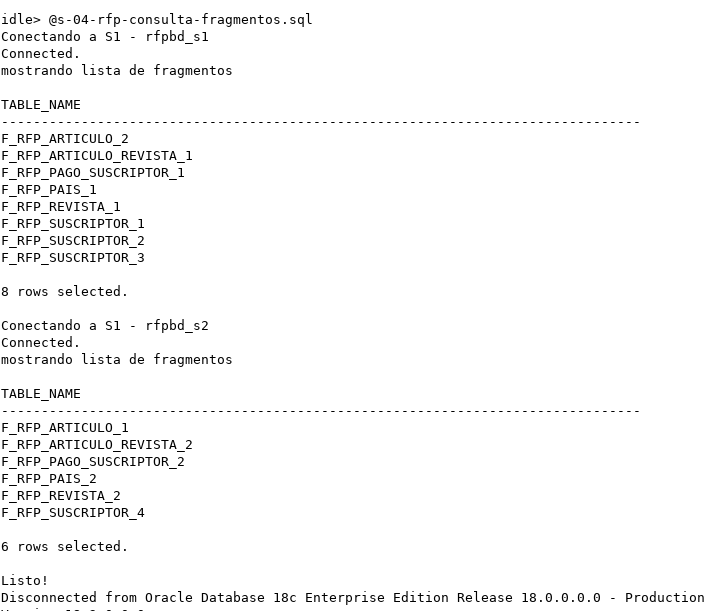
\includegraphics[width=0.8\linewidth]{bdd_prac05-c1-fragmentos}

\section*{C2. Código y salida del script 
\texttt{s-05-<iniciales>-consulta-restricciones-main.sql} y\\
\texttt{s-05-<iniciales>-consulta-restricciones.sql}}

\textbf{Restricciones main}

\lstinputlisting[language=SQL]
{bdd_prac_05-codigo/s-05-rfp-consulta-restricciones-main.sql}

\textbf{Restricciones}

\lstinputlisting[language=SQL]
{bdd_prac_05-codigo/s-05-rfp-consulta-restricciones.sql}

\textbf{Salida del archivo main del script anterior}\\
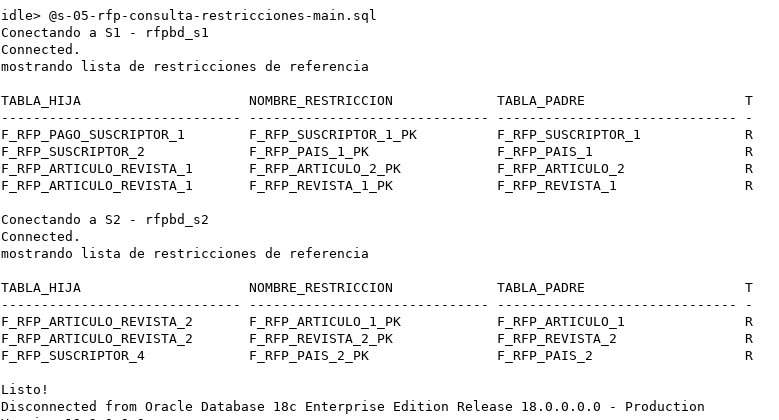
\includegraphics[width=0.8\linewidth]{bdd_prac05-c2-restricciones}

\section*{C3. Código y salida del script 
\texttt{s-07-<iniciales>-consultas.sql}}

\lstinputlisting[language=SQL]
{bdd_prac_05-codigo/s-07-rfp-consulta-datos.sql}

\newpage
\textbf{Salida del script anterior}\\
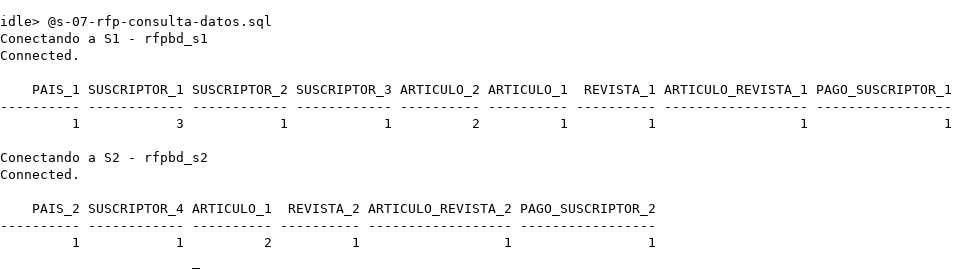
\includegraphics[width=\linewidth]{bdd_prac05-c3-consulta-datos}

\section*{C4. Salida de ejecución del script de validación 
\texttt{s-08-validacion-main.sql}}            

\textbf{Salida de Francisco Pablo Rodrigo}\\
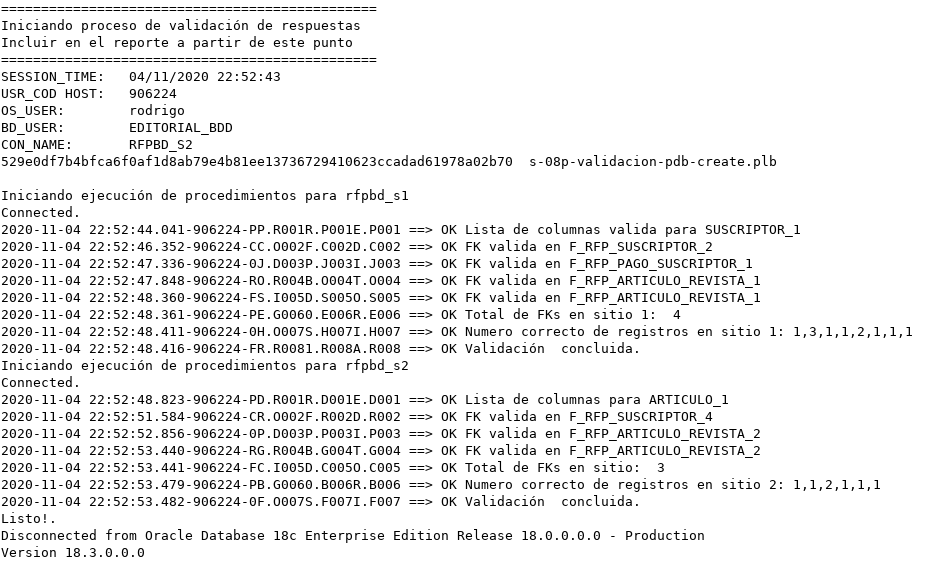
\includegraphics[width=\linewidth]{bdd_prac05-validador-rodrigo}

% \textbf{Salida de Francisco Martinez Emanuel}\\
% 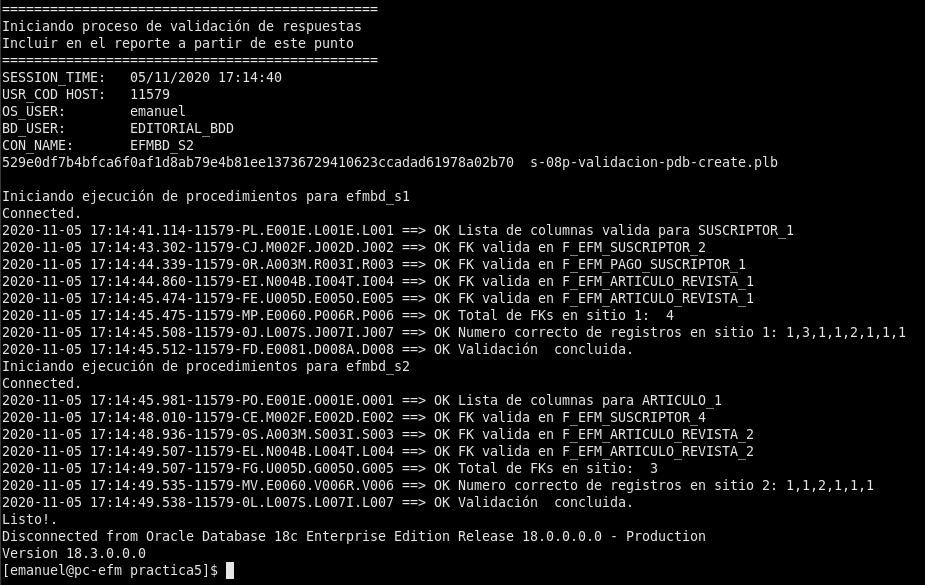
\includegraphics[width=\linewidth]{bdd_prac05-validador-emanuel}

\section*{Comentarios y conclusiones}

% TODO:- Agregar comentarios

\renewcommand\refname{Bibliografía}
\begin{thebibliography}{99}
    \bibitem{oracle} Oracle. \textit{Oracle Database Documentation} en 
        \texttt{https://docs.oracle.com/en/database/oracle/\\oracle-database/%
        index.html}
    %  TODO:- Add more references
\end{thebibliography}

\end{document}
